% !TeX program = xelatex
% Build from the project root: ./build.ps1 -Document 2/review.tex
\documentclass[12pt,a4paper]{article}
% !TeX root = ../2/main.tex
\usepackage[a4paper,margin=25mm,headheight=16pt]{geometry}
\usepackage{amsmath,amssymb}
\usepackage{graphicx}
\usepackage{booktabs}
\usepackage{tabularx}
\usepackage{siunitx}
\usepackage{tikz}
\usepackage{circuitikz}
\usepackage[unicode,hidelinks]{hyperref}
\usepackage{xepersian}
% Only the regular B Nazanin file is installed; synthesize bold explicitly.
\settextfont[Path=C:/Windows/Fonts/,AutoFakeBold=2,AutoFakeSlant=0.2]{B-NAZANIN.TTF}
% B Nazanin lacks U+066A (Arabic percent), required by xepersian's digit setup.
% Arial covers the complete required digit/punctuation set; Persian prose remains B Nazanin.
\setdigitfont[Path=C:/Windows/Fonts/,BoldFont=arialbd.ttf,ItalicFont=ariali.ttf,BoldItalicFont=arialbi.ttf]{arial.ttf}
\setmathdigitfont[Path=C:/Windows/Fonts/,BoldFont=arialbd.ttf,ItalicFont=ariali.ttf,BoldItalicFont=arialbi.ttf]{arial.ttf}
\setlatintextfont{TeX Gyre Termes}
% B Nazanin does not contain the default itemize bullet and dash glyphs.
\renewcommand{\labelitemi}{\(\bullet\)}
\renewcommand{\labelitemii}{\(\circ\)}
\renewcommand{\labelitemiii}{\(\diamond\)}
\setlength{\parindent}{0pt}
\setlength{\parskip}{0.5em}
\linespread{1.25}
\newcommand{\exercise}[1]{\section*{تمرین #1}}
% !TeX root = ../2/main.tex
% Shared title page for every assignment.
% Change only \AssignmentNumber and \AssignmentDate in each main document.

\newcommand{\AssignmentNumber}[1]{\gdef\assignmentnumber{#1}}
\newcommand{\AssignmentDate}[1]{\gdef\assignmentdate{#1}}

\newcommand{\assignmentnumber}{---}
\newcommand{\assignmentdate}{---}

% Stable course metadata
\newcommand{\universityname}{دانشگاه صنعتی امیرکبیر}
\newcommand{\universityalias}{پلی‌تکنیک تهران}
\newcommand{\facultyname}{دانشکده مهندسی کامپیوتر}
\newcommand{\coursename}{طراحی مدارهای مجتمع پرتراکم پیشرفته}
\newcommand{\studentname}{محمد خلیلی اصل}
\newcommand{\instructorname}{دکتر مهدی صدیقی}

\newcommand{\MakeAssignmentCover}{%
  \begin{titlepage}
    \thispagestyle{empty}
    \centering
    \linespread{1}\selectfont

    \vspace*{0mm}
    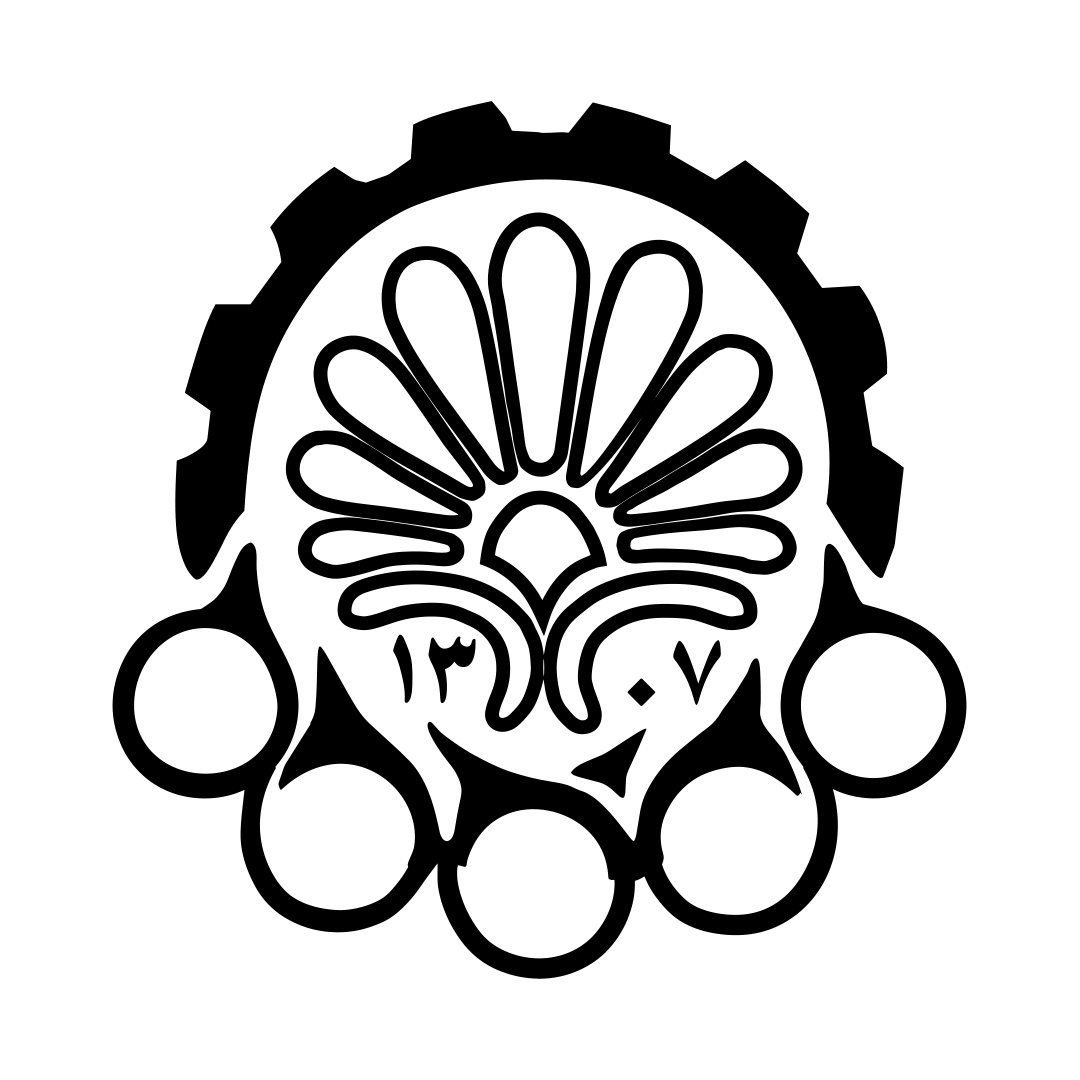
\includegraphics[width=44mm]{assets/aut-logo-black.png}\par
    \vspace{3mm}

    {\Large\bfseries \universityname\par}
    \vspace{1mm}
    {\large (\universityalias)\par}
    \vspace{1mm}
    {\large \facultyname\par}

    \vspace{8mm}
    {\Large\bfseries درس \coursename\par}

    \vspace{12mm}
    {\large عنوان\par}
    \vspace{2mm}
    {\LARGE\bfseries تمرین شماره \assignmentnumber\par}

    \vspace{10mm}
    {\large تهیه‌کننده\par}
    \vspace{2mm}
    {\Large\bfseries \studentname\par}

    \vspace{10mm}
    {\large استاد درس\par}
    \vspace{2mm}
    {\Large\bfseries \instructorname\par}

    \vspace{10mm}
    {\Large \assignmentdate\par}
    \vfill
  \end{titlepage}
  \setcounter{page}{1}%
}


% Preserve logical Unicode in PDF ActualText; do not paste shaped Arabic forms.
\XeTeXgenerateactualtext=1
% Keep dotted Persian identifiers in their intended order without changing font.
\newcommand{\exnum}[1]{\mbox{\beginL#1\endL}}
\newcommand{\reviewfile}[1]{\lr{\small\texttt{#1}}}
\newcommand{\bookpages}[2]{صفحات چاپی #1، صفحات #2 فایل \lr{PDF}}
\sisetup{per-mode=power}
\setlength{\emergencystretch}{2em}
\AssignmentNumber{۲}
\AssignmentDate{۲۰ آبان ۱۴۰۵}
\hypersetup{pdftitle={گزارش بررسی پاسخ‌های تمرین دوم},pdfauthor={محمد خلیلی اصل}}
\begin{document}
\MakeAssignmentCover

\section*{گزارش بررسی پاسخ‌های تمرین دوم}
\textbf{نتیجه کلی:} پاسخ‌های موجود، نتیجه اصلی هر هفت سؤال را به‌درستی تشخیص داده‌اند، اما مجموعه در وضعیت فعلی از نظر استدلال و ارائه کاملاً آماده تحویل نیست. مهم‌ترین خطا در روش دوم سؤال \exnum{۲.۲} است: حل معادله درجه‌دو نادرست است و به ولتاژ گره میانی ناسازگار با برابری جریان‌ها می‌رسد. در سؤال \exnum{۲.۷}، واحد یک ضریب فیزیکی اشتباه است؛ در سؤال \exnum{۲.۱۰}، افزایش جریان بدون فرض کافی به افزایش سرعت تعبیر شده است. چند توضیح نیز به تعیین دامنه اعتبار و ارجاع دقیق نیاز دارد.

\subsection*{دامنه و روش بررسی}
این گزارش هر هفت پاسخ \exnum{۲.۲}، \exnum{۲.۳} و \exnum{۲.۶} تا \exnum{۲.۱۰} را در فایل‌های \reviewfile{2/solutions/*.tex} و متن‌های اولیه \reviewfile{2/*.md} بررسی می‌کند. بازاجرای تبدیل موجود در حافظه، بدون نوشتن روی فایل‌ها، نشان داد محتوای هر هفت فایل \lr{LaTeX} با خروجی تبدیل پیش‌نویس متناظر یکسان است؛ بنابراین ایرادهای فنی به هر دو نسخه مربوط‌اند. فایل \reviewfile{2/main.tex} و خروجی موجود \reviewfile{build/main.pdf} نیز بررسی شدند. شماره خط‌های گزارش به نسخه بررسی‌شده اشاره دارند؛ پاسخ‌های اصلی در این بازبینی ویرایش نشده‌اند.

صورت سؤال‌ها و شکل \exnum{۲.۳۲} مستقیماً با کتاب \lr{Weste--Harris}، ویرایش چهارم، تطبیق داده شد \cite[\bookpages{۹۵ و ۹۶}{۱۲۲ و ۱۲۳}]{weste}. متن فارسی صورت هر هفت سؤال، داده‌ها و بخش‌های خواسته‌شده را درست منتقل کرده است. در صورت بازنویسی‌شده سؤال \exnum{۲.۲}، اشاره پرانتزی کتاب به برقرار بودن نتیجه در \lr{Saturation} حذف شده؛ اثبات صریح خواسته‌شده کتاب مربوط به \lr{Linear region} است و بررسی اشباع در این گزارش تکمیل‌کننده محسوب می‌شود. فهرست مستقل تکلیف استاد در پوشه موجود نیست؛ بنابراین درباره موظف بودن به حل سؤال‌های دیگر فصل، مانند \exnum{۲.۱}، \exnum{۲.۴} و \exnum{۲.۵}، داوری نشده است.

برای داوری، اسلایدهای مرتبط درس، معادلات کتاب، محاسبه مستقل، تحلیل ابعادی و شرایط ناحیه کار استفاده شد. شماره صفحات فایل \lr{PDF} در این گزارش از یک آغاز می‌شود؛ این شماره‌ها با شماره چاپی کتاب متفاوت‌اند. استخراج متن برخی منابع هشدار ساختار داخلی فایل داشت؛ صفحات اصلی سؤال‌ها، مدل سرعت و اسلایدهای کلیدی به‌صورت تصویری نیز خوانده شدند. نتیجه‌گیری بر پایه متن استخراج‌شده مخدوش یا شماره فایل حل‌المسائل انجام نشده است.

\subsection*{نمای کلی داوری}
جدول \ref{tab:verdict} وضعیت علمی پاسخ‌ها را خلاصه می‌کند. «تکمیل» به معنای نادرست بودن نتیجه اصلی نیست؛ محل و دلیل هر اصلاح در بخش همان سؤال آمده است.
\begin{table}[!htbp]
\centering
\caption{وضعیت پاسخ‌ها و اقدام لازم برای نسخه نهایی}
\label{tab:verdict}
\begin{tabularx}{\textwidth}{@{}r X X@{}}
\toprule
سؤال & داوری & اقدام لازم \\
\midrule
\exnum{۲.۲} & نتیجه و روش اول درست؛ روش دوم غلط & اصلاح ریشه، کنترل ناحیه کار و حذف نتیجه متناقض \\
\exnum{۲.۳} & پاسخ اصلی درست و کافی & تصریح بایاس مثبت و حالت برابری در جریان صفر \\
\exnum{۲.۶} & اثبات جبری درست & تکمیل مدل سرعت قطعه‌ای و محدود کردن ادعا به مدل \\
\exnum{۲.۷} & مقدار نهایی درست & اصلاح واحد ضریب بار و نگارش واحدهای سطحی \\
\exnum{۲.۸} & پاسخ «خیر» درست & تصریح فرض‌های حالت ماندگار و محدودیت زمانی \\
\exnum{۲.۹} & علامت بایاس و استدلال درست & ارجاع دقیق مثال‌های عددی و تفکیک سازوکارهای نشتی \\
\exnum{۲.۱۰} & هر سه ضریب عددی درست & اصلاح تعبیر سرعت، دمای مرجع و نماد ولتاژ آستانه \\
\bottomrule
\end{tabularx}
\end{table}

\section*{سؤال \exnum{۲.۲}: جریان دو ترانزیستور سری}
\subsection*{خواسته و ارزیابی پاسخ موجود}
خواسته، اثبات برابری جریان دو ترانزیستور \(W/L\) سری با جریان یک ترانزیستور \(W/(2L)\) در مدل \lr{Shockley} است. گیت‌ها به \(V_{DD}\) و سورس پایین به زمین متصل‌اند؛ \(V_{DD}>V_t\) و \(0\le V_{DS}<V_{DD}-V_t\) فرض می‌شود. تعریف \(\beta\)، ولتاژهای ترمینال و جمع کردن دو جریان در روش اول درست‌اند \cite[شکل \exnum{۲.۳۲}، صفحه چاپی ۹۵؛ روابط \exnum{۲.۵} تا \exnum{۲.۸}، صفحه چاپی ۶۶]{weste}.

\textbf{محل نخستین خطا:} در \reviewfile{2/solutions/2-2.tex}، خط ۹۸، ضریب اضافی ۲ زیر رادیکال وارد شده است. معادله درجه‌دو در خط ۹۵ درست است، ولی ریشه نوشته‌شده از آن به دست نمی‌آید. عبارت حاصل در خطوط ۱۰۱ تا ۱۰۵ عملاً \(V_1=V_{DS}\) است؛ در این صورت ولتاژ درین‌ـ‌سورس ترانزیستور بالا صفر و جریان آن صفر می‌شود، در حالی که جریان ترانزیستور پایین برای بایاس مثبت صفر نیست. عبارت «در تقریب درجه اول» این تناقض را رفع نمی‌کند؛ تقریب درست در ولتاژ کوچک \(V_1\approx V_{DS}/2\) است. پس خطا صرفاً تایپی یا تفاوت روش حل نیست.

\subsection*{حل صحیح و کنترل ریشه فیزیکی}
برای کوتاهی، \(A=V_{DD}-V_t>0\)، \(D=V_{DS}\)، \(x=V_1\) و \(\beta=\mu C_{\mathrm{ox}}W/L\) تعریف می‌کنیم. \(C_{\mathrm{ox}}\) ظرفیت اکسید بر واحد سطح و \(\mu\) تحرک حامل‌هاست. با فرض ثابت بودن \(V_t\)، صرف‌نظر از \lr{Body Effect} و \lr{Channel Length Modulation}، جریان ترانزیستور منفرد برابر است با
\begin{equation}
 I_{DS1}=\frac{\beta}{2}\left(AD-\frac{D^2}{2}\right).
 \label{eq:single}
\end{equation}
عامل \(\beta/2\) از دو برابر بودن طول کانال ناشی می‌شود. جریان‌های پایین و بالا، با فرض ناحیه خطی، به‌ترتیب عبارت‌اند از
\begin{align}
 I_{\mathrm{b}}&=\beta\left(Ax-\frac{x^2}{2}\right),\label{eq:bottom}\\
 I_{\mathrm{t}}&=\beta\left[(A-x)(D-x)-\frac{(D-x)^2}{2}\right]\notag\\
 &=\beta\left(AD-\frac{D^2}{2}-Ax+\frac{x^2}{2}\right).
 \label{eq:top}
\end{align}
در حالت ماندگار، قانون جریان گره میانی می‌دهد \(I_{\mathrm{b}}=I_{\mathrm{t}}=I_{DS2}\). با جمع روابط \eqref{eq:bottom} و \eqref{eq:top}، وابستگی به \(x\) حذف می‌شود:
\begin{equation}
 2I_{DS2}=\beta\left(AD-\frac{D^2}{2}\right)
 \quad\Longrightarrow\quad I_{DS2}=I_{DS1}.
 \label{eq:stack-equal}
\end{equation}
این همان بخش صحیح پاسخ موجود است. برای اجرای راهنمای کتاب و بررسی سازگاری فرض ناحیه کار، برابری دو جریان را حل می‌کنیم:
\begin{align}
 x^2-2Ax+AD-\frac{D^2}{2}&=0,\label{eq:quadratic}\\
 x&=A\pm\sqrt{A^2-AD+\frac{D^2}{2}}.\label{eq:roots}
\end{align}
در رابطه \eqref{eq:roots}، جمله ثابت معادله \eqref{eq:quadratic} فقط یک بار از \(A^2\) کم می‌شود. اگر \(0<D<A\)، رادیکال از \(A\) کوچک‌تر و از \(A-D\) بزرگ‌تر است، زیرا
\begin{equation}
 (A-D)^2<A^2-AD+\frac{D^2}{2}<A^2.
 \label{eq:root-range}
\end{equation}
بنابراین ریشه فیزیکی یکتا در بازه \(0<x<D\) برابر است با
\begin{equation}
 \boxed{V_1=A-\sqrt{A^2-AD+\frac{D^2}{2}}.}
 \label{eq:correct-v1}
\end{equation}
ریشه با علامت مثبت از \(A\) و در نتیجه از \(D\) بزرگ‌تر است و با ترتیب ولتاژ گره‌ها سازگار نیست. برای ریشه انتخاب‌شده، ترانزیستور پایین شرط \(x<A\) و ترانزیستور بالا شرط \(D-x<A-x\) را دارد؛ شرط دوم دقیقاً همان \(D<A\) است. هر دو ترانزیستور روشن و در ناحیه خطی‌اند. پس استفاده از روابط \eqref{eq:bottom} و \eqref{eq:top} نیز توجیه شده است.

\subsection*{کنترل‌های مستقل و تکمیل اشباع}
با بسط رابطه \eqref{eq:correct-v1} برای \(D/A\ll1\)، داریم
\begin{equation}
 V_1=\frac{D}{2}-\frac{D^2}{8A}
       +O\!\left(\frac{D^3}{A^2}\right).
 \label{eq:v1-small}
\end{equation}
در مرتبه اول افت ولتاژ تقریباً نصف می‌شود، نه برابر کل \(D\). به‌عنوان کنترل عددی فرضی، برای \(A=\qty{1}{\volt}\) و \(D=\qty{0.5}{\volt}\)، رابطه صحیح \(V_1\approx\qty{0.20943}{\volt}\) و \(I/\beta=\qty{0.1875}{\volt\squared}\) را در هر سه محاسبه می‌دهد. مقدار غلط \(V_1=\qty{0.5}{\volt}\) به \(I_{\mathrm{t}}=0\) و \(I_{\mathrm{b}}/\beta=\qty{0.375}{\volt\squared}\) می‌انجامد. این مثال داده فناوری نیست؛ فقط آزمون جبری است. در \(D=0\) نیز \(V_1=0\) و هر دو جریان صفرند.

برای تکمیل اشاره پرانتزی کتاب به \lr{Saturation}، اگر \(D\ge A\)، ترانزیستور بالا اشباع و ترانزیستور پایین خطی است. برابری جریان‌ها و ریشه فیزیکی می‌دهند
\begin{equation}
 \beta\left(Ax-\frac{x^2}{2}\right)=\frac{\beta}{2}(A-x)^2,
 \qquad x=A\left(1-\frac{1}{\sqrt{2}}\right).
 \label{eq:stack-sat}
\end{equation}
در این حالت \(x<A\) و \(D-x\ge A-x\) برقرار است و جریان برابر \(\beta A^2/4\) می‌شود؛ این مقدار دقیقاً جریان اشباع ترانزیستور \(W/(2L)\) است. نتیجه در مرز \(D=A\) پیوسته است. افزودن این بخش مفید است، اما خطای اصلی پاسخ موجود همان ریشه نادرست در ناحیه خطی است.

\section*{سؤال \exnum{۲.۳}: اثر بدنه در ساختار سری}
\subsection*{خواسته و داوری}
سؤال اثر \lr{Body Effect} را بر مقایسه جریان‌های سؤال قبل می‌خواهد. نتیجه \(I_{DS2}<I_{DS1}\) در پاسخ موجود صحیح است و توضیح افزایش آستانه ترانزیستور بالایی برای پاسخ کیفی سؤال کفایت می‌کند. در \reviewfile{2/solutions/2-3.tex}، خطوط ۵ تا ۷ و ۵۶، فقط بهتر است دامنه نامساوی روشن شود: این نامساوی سخت برای \(D>0\)، \(\gamma>0\) و بدنه‌های متصل به زمین است؛ در \(D=0\) هر دو جریان صفرند. این نکته تکمیل شرایط مرزی است و نتیجه اصلی را رد نمی‌کند.

\subsection*{استدلال صحیح و اثبات کاهش جریان}
رابطه آستانه با اثر بدنه در کتاب و اسلاید درس یکسان است \cite[بخش \exnum{۲.۴.۳.۱}، صفحه چاپی ۷۹، صفحه ۱۰۶ فایل]{weste}\cite[اسلایدهای ۱۶ و ۱۷]{nonideal}:
\begin{equation}
 V_t=V_{t0}+\gamma\left(\sqrt{\phi_s+V_{SB}}-\sqrt{\phi_s}\right).
 \label{eq:body}
\end{equation}
در این رابطه، \(V_{t0}\) آستانه در بایاس صفر سورس‌ـ‌بدنه، \(\gamma>0\) ضریب اثر بدنه و \(\phi_s>0\) پتانسیل سطحی در آستانه است. برای ترانزیستور منفرد و ترانزیستور پایین \(V_{SB}=0\) است. برای ترانزیستور بالا، با \(x=V_1>0\)، افزایش آستانه برابر است با
\begin{equation}
 \delta(x)=\gamma\left(\sqrt{\phi_s+x}-\sqrt{\phi_s}\right)>0.
 \label{eq:delta-body}
\end{equation}
پس در یک ولتاژ میانی ثابت، جریان ترانزیستور بالا کم می‌شود. گره میانی سپس جابه‌جا می‌شود تا جریان بالا و پایین دوباره یکسان شوند؛ این جابه‌جایی باید در استدلال لحاظ شود.

برای اثبات، \(A=V_{DD}-V_{t0}\) و \(0<D<A\) را در نظر می‌گیریم. \(x_0\) ریشه صحیح سؤال قبل است. جریان پایین \(f(x)=\beta(Ax-x^2/2)\) در \(0<x<D\) صعودی است، زیرا \(f'(x)=\beta(A-x)>0\). جریان بالای بدون اثر بدنه، یعنی \(g_0(x)\) در رابطه \eqref{eq:top}، نزولی است. افزودن \(\delta(x)\) جریان بالا را در هر \(x>0\) کاهش می‌دهد. بنابراین در \(x=x_0\)، جریان بالا از جریان پایین کمتر می‌شود. برای \(x\ge x_0\) نیز برابری ممکن نیست، زیرا \(f\) افزایش و جریان بالا کاهش یافته است؛ نقطه کار جدید باید \(x_{\mathrm{BE}}<x_0\) باشد. در نتیجه
\begin{equation}
 I_{DS2,\mathrm{BE}}=f(x_{\mathrm{BE}})<f(x_0)=I_{DS1}.
 \label{eq:body-inequality}
\end{equation}
این برهان حتی اگر ترانزیستور بالا پس از افزایش آستانه وارد اشباع شود معتبر است: در مدل \lr{Shockley}، کاهش \lr{Gate Overdrive} در ولتاژ درین‌ـ‌سورس ثابت، جریان را در هر دو ناحیه کاهش می‌دهد. پس نباید بی‌بررسی فرض کرد شرط خطی بودن آن پس از افزودن اثر بدنه هم برقرار می‌ماند.

اگر هر دو ترانزیستور همچنان خطی باشند، جمع جریان‌ها یک نمایش مستقیم‌تر از کاهش جریان می‌دهد:
\begin{equation}
 I_{DS2,\mathrm{BE}}=I_{DS1}-\frac{\beta}{2}\delta(x)(D-x)<I_{DS1}.
 \label{eq:body-linear}
\end{equation}
شرط استفاده از رابطه \eqref{eq:body-linear} برای ترانزیستور بالا \(D<A-\delta(x)\) است. این رابطه با علامت مثبت \(\delta(x)\) و \(D-x\)، جهت تغییر را تأیید می‌کند. بنابراین پاسخ موجود از نظر خواسته اصلی درست است؛ برهان حاضر جایگاه دقیق تغییر نقطه کار و شرایط مرزی را تکمیل می‌کند.

\section*{سؤال \exnum{۲.۶}: اثبات ولتاژ شروع اشباع}
\subsection*{خواسته و داوری پاسخ}
کتاب اثبات رابطه \exnum{۲.۲۷} را می‌خواهد. هم معادله نهایی و هم مراحل برابرسازی دو شاخه جریان در \reviewfile{2/solutions/2-6.tex} درست‌اند؛ حذف جمله‌های درجه‌دو نیز خطا نیست. دو نکته در مقدمه و تفسیر باید اصلاح شوند.

نخست، رابطه سرعت در خط ۲۰ فقط شاخه \(E<E_c\) مدل قطعه‌ای کتاب است. اگر این عبارت بدون شرط به همه میدان‌ها تعمیم یابد، حد آن \(\mu_{\mathrm{eff}}E_c=2v_{\mathrm{sat}}\) خواهد بود، نه \(v_{\mathrm{sat}}\). مدل کامل کتاب در صفحه چاپی ۷۶ و اسلاید ۹، برای \(E\ge E_c\) شاخه ثابت دارد \cite[روابط \exnum{۲.۲۴} و \exnum{۲.۲۵}]{weste}\cite[اسلاید ۹]{nonideal}. دوم، عبارت \(C_{\mathrm{ox}}W(V_{GT}-V_{\mathrm{dsat}})\) در خط ۳۰ بار کل کانال نیست؛ بعد آن بار بر واحد طول است. نام دقیق آن را می‌توان \(q'_{\mathrm{inv,d}}\)، قدرمطلق بار وارونگی بر واحد طول در انتهای درین، گذاشت. ضرب این کمیت در سرعت، بعد جریان دارد.

\subsection*{اثبات صحیح در مدل کتاب}
\(A=V_{GT}=V_{gs}-V_t>0\)، \(s=V_{\mathrm{dsat}}\) و \(V_c=E_cL>0\) را تعریف می‌کنیم. \(E\) میدان جانبی، \(v\) سرعت رانش و \(\mu_{\mathrm{eff}}\) تحرک مؤثر است. مدل سرعت و شرط پیوستگی آن عبارت‌اند از
\begin{equation}
 v(E)=
 \begin{cases}
 \dfrac{\mu_{\mathrm{eff}}E}{1+E/E_c},&0\le E<E_c,\\[4pt]
 v_{\mathrm{sat}},&E\ge E_c,
 \end{cases}
 \qquad E_c=\frac{2v_{\mathrm{sat}}}{\mu_{\mathrm{eff}}}.
 \label{eq:velocity}
\end{equation}
مطابق رابطه \exnum{۲.۲۶} کتاب، دو شاخه جریان باید در \(V_{ds}=s\) پیوسته باشند \cite[صفحه چاپی ۷۷، صفحه ۱۰۴ فایل]{weste}. از \(v_{\mathrm{sat}}=\mu_{\mathrm{eff}}V_c/(2L)\) استفاده می‌کنیم و می‌نویسیم
\begin{equation}
 \frac{\mu_{\mathrm{eff}}C_{\mathrm{ox}}W}{L}
 \frac{(A-s/2)s}{1+s/V_c}
 =C_{\mathrm{ox}}W(A-s)\frac{\mu_{\mathrm{eff}}V_c}{2L}.
 \label{eq:velocity-match}
\end{equation}
پس از حذف عوامل مشترک مثبت و ضرب در \(2(V_c+s)/V_c\)، رابطه به صورت زیر ساده می‌شود:
\begin{align}
 2As-s^2&=(A-s)(V_c+s),\notag\\
 2As-s^2&=AV_c+As-V_cs-s^2,\notag\\
 (A+V_c)s&=AV_c.
 \label{eq:velocity-algebra}
\end{align}
ازاین‌رو جواب دقیق در این مدل برابر است با
\begin{equation}
 \boxed{V_{\mathrm{dsat}}=\frac{V_{GT}V_c}{V_{GT}+V_c}.}
 \label{eq:vdsat}
\end{equation}
این دقیقاً نتیجه پاسخ موجود و رابطه مورد درخواست است. عبارت «دقیق» در اینجا به حل جبری مدل اشاره دارد، نه به توصیف کامل هر ترانزیستور واقعی.

\subsection*{دامنه اعتبار و حدها}
برای \(V_{GT},V_c>0\)، رابطه \eqref{eq:vdsat} از هر دو مقدار \(V_{GT}\) و \(V_c\) کوچک‌تر است. اگر \(V_c\gg V_{GT}\)، آنگاه \(V_{\mathrm{dsat}}\approx V_{GT}\)؛ اگر \(V_{GT}\gg V_c\)، آنگاه \(V_{\mathrm{dsat}}\approx V_c\). حد اول بازگشت به مدل کانال بلند و حد دوم غلبه \lr{Velocity Saturation} است. در حد دوم، جایگذاری در شاخه اشباع کتاب می‌دهد
\begin{equation}
 I_{\mathrm{dsat}}=
 C_{\mathrm{ox}}Wv_{\mathrm{sat}}\frac{V_{GT}^2}{V_{GT}+V_c}
 \approx C_{\mathrm{ox}}Wv_{\mathrm{sat}}V_{GT}.
 \label{eq:velocity-current}
\end{equation}
در خطوط ۱۰۲ و ۱۰۵ پاسخ، استقلال از ولتاژ گیت و عبارت «در تمام ترانزیستورهای عملی نانومتری» بیش از دامنه مدل ادعا می‌کنند. بیان درست این است: «در این مدل، برای پارامترهای مثبت، \(V_{\mathrm{dsat}}<\min(V_{GT},V_c)\)؛ در حد غلبه اشباع سرعت و با ثابت گرفتن \(V_c\)، حساسیت آن به \(V_{GT}\) کم می‌شود.» خود کتاب تصریح می‌کند \(\mu_{\mathrm{eff}}\) می‌تواند با \(V_{gs}\) تغییر کند؛ بنابراین \(V_c=2v_{\mathrm{sat}}L/\mu_{\mathrm{eff}}\) لزوماً مستقل از گیت نیست. این اصلاحات، اثبات جبری صحیح را تغییر نمی‌دهند.

\section*{سؤال \exnum{۲.۷}: تغییر عددی ولتاژ آستانه}
\subsection*{خواسته و نتیجه بررسی}
داده‌های پاسخ با سؤال کتاب یکسان‌اند: ضخامت اکسید \qty{10}{\nano\metre}، غلظت ناخالصی \(N_A=\qty{2e17}{\per\cubic\centi\metre}\)، آستانه اولیه \qty{0.7}{\volt}، بدنه در زمین و افزایش ولتاژ سورس از صفر به \qty{4}{\volt}. تبدیل ضخامت از آنگستروم به سانتی‌متر درست است. مقدار \(\Delta V_t\approx\qty{0.954}{\volt}\) و آستانه جدید \(V_t\approx\qty{1.654}{\volt}\) نیز تأیید می‌شوند.

\textbf{ایراد مشخص:} در \reviewfile{2/solutions/2-7.tex}، خط ۷۷، واحد \(\sqrt{2q\varepsilon_{\mathrm{si}}N_A}\) به‌صورت بار بر واحد سطح نوشته شده است. این کمیت هنوز در ریشه ولتاژ ضرب نشده؛ واحد صحیح آن \(\unit{\coulomb\per\square\centi\metre\per\volt\tothe{0.5}}\) است. عبارت توضیحی «به ازای پتانسیل یک ولت» تنها وقتی واحد بار سطحی می‌دهد که عامل \(\sqrt{\qty{1}{\volt}}\) واقعاً در کمیت منظور شود. در فرمول چاپ‌شده چنین عاملی وجود ندارد. همچنین در خطوط ۷۳ و ۷۷، توان ۲ بیرون از کل متن واحد قرار گرفته است؛ بهتر است \(C_{\mathrm{ox}}\) به‌صراحت با واحد \(\unit{\farad\per\square\centi\metre}\) نوشته شود تا توان فقط به طول مربوط باشد.

\subsection*{محاسبه مستقل با ثابت‌های کتاب}
برای سازگاری با مثال \exnum{۲.۵} کتاب، از \(v_T=\qty{0.026}{\volt}\)، \(n_i=\qty{1.45e10}{\per\cubic\centi\metre}\)، \(q=\qty{1.6e-19}{\coulomb}\) و \(\varepsilon_0=\qty{8.85e-14}{\farad\per\centi\metre}\) استفاده می‌کنیم. \(n_i\) غلظت ذاتی حامل‌ها و \(q\) قدرمطلق بار الکترون است. گذردهی‌ها \(\varepsilon_{\mathrm{ox}}=3.9\varepsilon_0\) و \(\varepsilon_{\mathrm{si}}=11.7\varepsilon_0\) هستند \cite[صفحات چاپی ۶۵ و ۷۹ تا ۸۰]{weste}. رابطه اثر بدنه و تعریف پارامترها در اسلایدهای ۱۶ و ۱۷ نیز آمده‌اند \cite{nonideal}.

ابتدا \(V_{SB}=\qty{4}{\volt}\) و \(t_{\mathrm{ox}}=\qty{1e-6}{\centi\metre}\) است. پتانسیل سطحی از رابطه کتاب به دست می‌آید:
\begin{equation}
 \phi_s=2v_T\ln\!\left(\frac{N_A}{n_i}\right)
 =2(\qty{0.026}{\volt})\ln\!\left(\frac{2\times10^{17}}{1.45\times10^{10}}\right)
 \approx\qty{0.85486}{\volt}.
 \label{eq:phi}
\end{equation}
ظرفیت اکسید بر واحد سطح و ضریب بار برابرند با
\begin{align}
 C_{\mathrm{ox}}&=\frac{\varepsilon_{\mathrm{ox}}}{t_{\mathrm{ox}}}
 =\qty{3.4515e-7}{\farad\per\square\centi\metre},\label{eq:cox}\\
 B&\equiv\sqrt{2q\varepsilon_{\mathrm{si}}N_A}
 \approx\qty{2.57427e-7}{\coulomb\per\square\centi\metre\per\volt\tothe{0.5}}.
 \label{eq:body-coefficient}
\end{align}
نماد \(B\) در اینجا تنها برای ضریب زیر رادیکال تعریف شده و ولتاژ بدنه نیست. کنترل ابعادی علت اصلاح واحد را نشان می‌دهد:
\begin{equation}
 [B]=\sqrt{\unit{\coulomb}\,
                \unit{\farad\per\centi\metre}\,
                \unit{\per\cubic\centi\metre}}
 =\unit{\coulomb\per\square\centi\metre\per\volt\tothe{0.5}}.
 \label{eq:dimension}
\end{equation}
با استفاده از \(\unit{\farad}=\unit{\coulomb\per\volt}\)، بعد \(B/C_{\mathrm{ox}}\) ریشه ولتاژ است؛ بنابراین
\begin{equation}
 \gamma=\frac{B}{C_{\mathrm{ox}}}
 \approx\qty{0.74584}{\volt\tothe{0.5}}.
 \label{eq:gamma}
\end{equation}
جایگذاری روابط \eqref{eq:phi} و \eqref{eq:gamma} در رابطه \eqref{eq:body}، بدون گرد کردن زودهنگام، می‌دهد
\begin{align}
 \Delta V_t&=\gamma\left(\sqrt{\phi_s+\qty{4}{\volt}}-\sqrt{\phi_s}\right)
 \approx\qty{0.95377}{\volt},\label{eq:threshold-shift}\\
 V_t&=\qty{0.7}{\volt}+\Delta V_t\approx\qty{1.65377}{\volt}.
 \label{eq:threshold-new}
\end{align}
ارقام اضافی فقط برای بازتولید محاسبه‌اند؛ برای گزارش نهایی، \(\boxed{\Delta V_t\approx\qty{0.95}{\volt},\quad V_t\approx\qty{1.65}{\volt}}\) با دقت داده‌ها سازگار است. این \(V_t\) ولتاژ گیت نسبت به سورس در آستانه است، نه ولتاژ گیت نسبت به زمین. بنابراین بالا رفتن خود سورس به \qty{4}{\volt} نباید دوباره به \(\Delta V_t\) اضافه شود.

\subsection*{کنترل تقریب خطی}
پاسخ موجود به‌درستی استفاده از تقریب خطی را برای این بایاس رد می‌کند. شیب در بایاس صفر برابر است با
\begin{equation}
 k_\gamma=\frac{\gamma}{2\sqrt{\phi_s}}\approx0.40334,
 \qquad \Delta V_{t,\mathrm{lin}}=k_\gamma V_{SB}\approx\qty{1.61}{\volt}.
 \label{eq:body-small-signal}
\end{equation}
شرط خطی‌سازی \(V_{SB}\ll\phi_s\) در این مثال برقرار نیست؛ نسبت آن‌ها حدود \num{4.7} است. تابع ریشه دوم مقعر است، پس خط مماس در صفر افزایش آستانه را بیش‌برآورد می‌کند. به همین دلیل جواب کامل \qty{0.95}{\volt} معتبر است و مقدار \qty{1.61}{\volt} نباید جواب سؤال قرار گیرد. خطای واحد در مرحله میانی، با وجود ضروری بودن اصلاح، محاسبه عددی نهایی را خراب نکرده است.

\section*{سؤال \exnum{۲.۸}: تعداد ترانزیستورهای سری}
\subsection*{خواسته و داوری}
سؤال می‌پرسد آیا خود \lr{Body Effect} در فرکانس پایین، حدی برای تعداد ترانزیستورهای سری در گیت \lr{CMOS} تعیین می‌کند. پاسخ «خیر» درست است. استدلال تخلیه گره‌های میانی در \reviewfile{2/solutions/2-8.tex} نیز جهت درستی دارد، اما عبارت‌های «تعداد نامحدود» و «تمام گره‌ها دقیقاً صفر می‌شوند» در خطوط ۱۳ و ۲۳ به تصریح مدل نیاز دارند.

صورت دقیق نتیجه این است: برای هر تعداد \textbf{متناهی} ترانزیستور، در یک گیت \lr{Static CMOS} با تغذیه مناسب و فرصت کافی برای رسیدن به حالت ماندگار، اثر بدنه به‌تنهایی حد سختی بر تعداد سری تعیین نمی‌کند. این گفته تضمین نمی‌کند که یک فرکانس ثابت، هرچند پایین، برای هر تعداد دلخواه کافی باشد. همچنین در مدار واقعی، جریان بار یا نشتی مسیر مقابل می‌تواند افت ولتاژ کوچکی ایجاد کند؛ صفر شدن دقیق همه گره‌ها نتیجه مدل بدون آن جریان‌هاست.

\subsection*{استدلال کامل}
شبکه \lr{Pull-Down} شامل \(N\) ترانزیستور \lr{nMOS} با بدنه متصل به زمین را در نظر می‌گیریم. همه ورودی‌ها یک و \(V_{DD}>V_{t0}\) است؛ شبکه \lr{Pull-Up} خاموش و خروجی در حالت ماندگار بدون جریان بار فرض می‌شود. ترانزیستور پایین به زمین وصل است و می‌تواند گره بالای خود را تخلیه کند. با افت این گره، \(V_{SB}\) ترانزیستور بعدی کاهش و \(V_{GS}\) آن افزایش می‌یابد؛ مسیر تخلیه برای گره‌های بالاتر نیز برقرار می‌شود. در حالت نهایی بدون جریان خارجی، افت ولتاژ روی هر ترانزیستور روشن صفر است، پس
\begin{equation}
 V_{S,i}\longrightarrow0,\qquad V_{SB,i}\longrightarrow0,
 \qquad V_{t,i}\longrightarrow V_{t0}\qquad (i=1,\ldots,N).
 \label{eq:stack-dc}
\end{equation}
اثر بدنه در طول گذار جریان را کم می‌کند، اما در این حالت نهایی مانع رساندن صفر قوی نمی‌شود. استدلال دوگان برای شبکه \lr{pMOS} با بدنه متصل به \(V_{DD}\)، رساندن یک قوی را نتیجه می‌دهد. در این تحلیل، منشأ تخلیه هدایت شبکه روشن است؛ نیازی نیست نشتی را علت ضروری تخلیه بدانیم. رفتار رساندن سطح قوی در کتاب و مبانی ترانزیستور درس توضیح داده شده است \cite[بخش \exnum{۲.۵.۴} و خلاصه فصل در صفحه چاپی ۹۵]{weste}\cite[اسلایدهای ۶ تا ۱۳]{mosfet}.

\subsection*{محدودیت عملی و اعتبار ادعاهای اضافه}
ادعای رشد درجه‌دو تأخیر و توصیه چهار یا پنج ترانزیستور، برخلاف یک ادعای بدون پشتوانه، در کتاب وجود دارد. با مدل اندازه‌گذاری و ظرفیت‌های شکل \exnum{۴.۲۳}، رابطه \exnum{۴.۲۳} کتاب می‌دهد
\begin{equation}
 t_{pd}=\left(\frac{N^2}{2}+\frac{5N}{2}\right)RC.
 \label{eq:elmore}
\end{equation}
در این مدل، مقاومت هر ترانزیستور سری \(R/N\)، ظرفیت هر گره داخلی \(NC\) و ظرفیت خروجی \(3NC\) است. رشد درجه‌دو از همین فرض‌ها و الگوی گذار شکل نتیجه می‌شود؛ قانون دقیق و مستقل از بار و اندازه‌گذاری برای همه مدارها نیست \cite[\bookpages{۱۵۷ و ۱۵۸}{۱۸۴ و ۱۸۵}]{weste}. کتاب می‌گوید ساخت گیت با بیش از چهار یا احتمالاً پنج ترانزیستور سری معمولاً توصیه نمی‌شود؛ این توصیه کارایی است، نه ممنوعیت فیزیکی. بنابراین بخش اضافه پاسخ قابل حفظ است، به شرط ارجاع و بیان همین محدودیت‌ها.

\section*{سؤال \exnum{۲.۹}: علامت بایاس بدنه}
\subsection*{خواسته و پاسخ صحیح}
سؤال فقط علامت بایاس لازم برای افزایش آستانه \lr{nMOS} را می‌خواهد. پاسخ موجود «بایاس منفی بدنه» برای سورس در زمین درست است و استدلال جبری آن سؤال را کامل پاسخ می‌دهد. بیان عمومی‌تر، پایین آوردن پتانسیل بدنه نسبت به سورس است؛ منفی بودن مطلق ولتاژ تنها وقتی لازم است که سورس مرجع صفر باشد.

با ثابت بودن \(V_S\) و با \(V_{SB}=V_S-V_B\)، مشتق رابطه \eqref{eq:body} نشان می‌دهد
\begin{equation}
 \frac{\partial V_t}{\partial V_B}
 =-\frac{\gamma}{2\sqrt{\phi_s+V_S-V_B}}<0.
 \label{eq:body-bias-derivative}
\end{equation}
پس کاهش \(V_B\) آستانه را بالا می‌برد؛ در حالت \(V_S=0\)، انتخاب \(V_B<0\) یا \lr{Reverse Body Bias} لازم است. افزایش بایاس معکوس، قدرمطلق بار تخلیه زیر گیت را بیشتر می‌کند و برای تشکیل کانال به ولتاژ گیت بالاتری نیاز است \cite[رابطه \exnum{۲.۳۵}، صفحه چاپی ۷۹]{weste}\cite[اسلاید ۱۶]{nonideal}.

اگر فرمول بار تخلیه پاسخ موجود حفظ شود، باید \(Q_{\mathrm{dep}}\) در خط ۴۶ \reviewfile{2/solutions/2-9.tex} به‌صراحت \textbf{بار بر واحد سطح} تعریف شود:
\begin{equation}
 |Q_{\mathrm{dep}}|=\sqrt{2q\varepsilon_{\mathrm{si}}N_A(\phi_s+V_{SB})}.
 \label{eq:depletion-charge}
\end{equation}
در رابطه \eqref{eq:depletion-charge}، \(q\) قدرمطلق بار الکترون، \(\varepsilon_{\mathrm{si}}\) گذردهی سیلیکون و \(N_A\) غلظت ناخالصی پذیرنده است. واحد این بار سطحی \(\unit{\coulomb\per\square\centi\metre}\) است؛ بر خلاف ضریب فاقد ریشه ولتاژ در سؤال قبل. نتیجه افزایش آستانه به محاسبه عددی یا تعیین یک بایاس مشخص وابسته نیست.

\subsection*{بررسی دقیق مثال‌های اضافه و اصلاح پیشنهادی}
در بخش کاربرد پاسخ، دو عدد \qty{-0.4}{\volt} و \qty{-1.2}{\volt} آمده است. این اعداد ساختگی نیستند: هر دو در بخش \exnum{۵.۳.۴} کتاب، صفحه چاپی ۲۰۰، وجود دارند. مقدار \qty{-0.4}{\volt} در یک مثال فناوری \qty{1}{\volt} بیان شده و مقدار منفی‌تر از \qty{-1.2}{\volt} مثال افزایش \lr{Junction Leakage} از راه \lr{Band-to-Band Tunneling (BTBT)} است \cite[صفحه ۲۲۷ فایل]{weste}. بنابراین ایراد درست به این بخش، «بی‌منبع بودن خود اعداد» نیست؛ مشکل، نبود ارجاع و جدا شدن آن‌ها از شرایط مثال است. هیچ‌یک از این دو مقدار حد مجاز عمومی فناوری‌های \lr{CMOS} نیست.

در خط ۶۳ پاسخ، \lr{BTBT}، شکست پیوند و \lr{Gate-Induced Drain Leakage (GIDL)} در یک توضیح کلی جمع شده‌اند. \lr{BTBT} نباید بدون تفکیک، همان شکست بهمنی پیوند تلقی شود. افزون بر این، توضیح کتاب برای مثال بایاس بدنه بر نشتی پیوند از راه \lr{BTBT} متمرکز است؛ بحث \lr{GIDL} در بخش \exnum{۲.۴.۴.۳} و اسلاید ۲۸ به میدان شدید نزدیک درین، به‌ویژه درین مثبت و گیت منفی، مربوط است \cite[صفحات چاپی ۸۴ و ۲۰۰]{weste}\cite[اسلاید ۲۸]{nonideal}. برای افزودن اثر بایاس بدنه بر آن باید شرایط بایاس و مدل مشخص باشد.

متن جایگزین مناسب چنین است: «\lr{Reverse Body Bias} آستانه را افزایش و مؤلفه نشتی زیرآستانه را کاهش می‌دهد. افزایش بیش از حد آن ممکن است نشتی پیوند ناشی از \lr{BTBT} را بیشتر کند و مزیت کاهش نشتی را محدود سازد. مقادیر نمونه کتاب به فناوری و بایاس مثال مربوط‌اند و برای تعیین حد مجاز یک فرایند مشخص کافی نیستند.» این اصلاح فقط توضیح تکمیلی را دقیق‌تر می‌کند؛ پاسخ اصلی علامت بایاس درست است.

\section*{سؤال \exnum{۲.۱۰}: کاهش آستانه، جریان روشن و نشتی}
\subsection*{خواسته و فرض‌های مشترک}
هر سه بخش صورت سؤال درست منتقل و پاسخ داده شده‌اند: کاهش آستانه از \qty{0.4}{\volt} به \qty{0.3}{\volt} در \(V_{DD}=\qty{1.2}{\volt}\)، ضریب افزایش جریان اشباع ایده‌آل، ضریب افزایش نشتی در دمای اتاق و همان مقایسه در \qty{120}{\degreeCelsius}. در بخش ج، نسبت مورد نظر بین دو آستانه \textbf{در همان دمای بالا} است، نه نسبت نشتی دمای بالا به دمای اتاق. تفسیر فعلی پاسخ از این بخش درست است.

برای این مقایسه مدل‌شده، ابعاد، \(\beta\)، ضریب \(n=1.4\)، بایاس‌ها و سایر پارامترها در مقایسه دو آستانه در یک دمای ثابت یکسان فرض می‌شوند. وابستگی خود آستانه به دما نیز طبق صورت سؤال نادیده گرفته می‌شود. در فناوری واقعی تغییر فرایند برای کاهش آستانه می‌تواند پارامترهای دیگر را هم تغییر دهد؛ چنین مدلی در سؤال داده نشده است.

\subsection*{حل بخش الف: جریان اشباع}
در مدل \lr{Shockley}، \(I_{\mathrm{sat}}=\beta(V_{GS}-V_t)^2/2\) است \cite[رابطه \exnum{۲.۸}، صفحه چاپی ۶۶]{weste}. برای هر دو آستانه، شرط اشباع برقرار است، زیرا \(V_{DS}=\qty{1.2}{\volt}\) از \qty{0.8}{\volt} و \qty{0.9}{\volt} بزرگ‌تر است. نسبت جدید به قدیم برابر است با
\begin{equation}
 r_{\mathrm{on}}=\frac{I_{\mathrm{sat,new}}}{I_{\mathrm{sat,old}}}
 =\left(\frac{1.2-0.3}{1.2-0.4}\right)^2
 =\frac{81}{64}=1.265625\approx1.27.
 \label{eq:on-ratio}
\end{equation}
پس جریان اشباع حدود \num{26.6} درصد افزایش می‌یابد. این نتیجه عددی پاسخ موجود صحیح است.

\subsection*{حل بخش‌های ب و ج: نسبت نشتی در یک دمای ثابت}
در رابطه عمومی \exnum{۲.۴۲} کتاب، آستانه مرجع \(V_{t0}\) است؛ اثر \lr{DIBL} و اثر بدنه جداگانه وارد می‌شوند \cite[صفحات چاپی ۸۱ و ۸۲، صفحات ۱۰۸ و ۱۰۹ فایل]{weste}\cite[اسلاید ۲۳]{nonideal}:
\begin{equation}
 I_{\mathrm{sub}}=I_{ds0}
 \exp\!\left(\frac{V_{GS}-V_{t0}+\eta V_{DS}-k_\gamma V_{SB}}{nv_T}\right)
 \left(1-\exp\!\left[-\frac{V_{DS}}{v_T}\right]\right).
 \label{eq:subthreshold}
\end{equation}
در این مدل، \(I_{ds0}\) ضریب جریان وابسته به هندسه و فرایند، \(\eta\) ضریب \lr{Drain-Induced Barrier Lowering (DIBL)}، \(k_\gamma\) حساسیت خطی آستانه به \(V_{SB}\)، \(n\) ضریب شیب زیرآستانه و \(v_T=kT/q\) ولتاژ حرارتی است. \(k\) ثابت بولتزمن و \(T\) دمای مطلق است. با \(V_{GS}=0\)، بایاس و ضرایب یکسان، و \(\Delta V_t=V_{t,\mathrm{old}}-V_{t,\mathrm{new}}=\qty{0.1}{\volt}\)، عوامل مشترک در نسبت حذف می‌شوند:
\begin{equation}
 r_{\mathrm{sub}}(T)=
 \frac{I_{\mathrm{sub,new}}(T)}{I_{\mathrm{sub,old}}(T)}
 =\exp\!\left(\frac{\Delta V_t}{nv_T(T)}\right).
 \label{eq:leak-ratio}
\end{equation}
برای این حذف، حتی لازم نیست \(\eta\) را صفر بگیریم؛ ثابت بودن اثر آن در دو حالت کافی است. حذف ضریب \(I_{ds0}\) نیز فقط در مقایسه دو آستانه در یک دمای ثابت و با فرض یکسان بودن آن مجاز است.

در بخش ب، با تقریب دمای اتاق کتاب یعنی \(v_T\approx\qty{26}{\milli\volt}\)، نتیجه چنین است:
\begin{equation}
 r_{\mathrm{sub,room}}=
 \exp\!\left(\frac{0.100}{1.4\times0.026}\right)
 \approx15.60.
 \label{eq:leak-room}
\end{equation}
برای کنترل مستقل، \lr{Subthreshold Slope} برابر \(S=nv_T\ln10\approx\qty{83.8}{\milli\volt}\) به ازای یک دهه تغییر جریان است. بنابراین \(10^{100/83.8}\approx15.6\)، همان جواب را می‌دهد.

در بخش ج، \(T=\qty{393.15}{\kelvin}\) و \(v_T\approx\qty{33.879}{\milli\volt}\) است. با تقریب کتاب \(v_T\approx\qty{34}{\milli\volt}\)، داریم
\begin{equation}
 r_{\mathrm{sub,hot}}=
 \exp\!\left(\frac{0.100}{1.4\times0.034}\right)
 \approx8.17\approx8.2.
 \label{eq:leak-hot}
\end{equation}
استفاده از مقدار گردنشده ولتاژ حرارتی، نسبت حدود \num{8.23} می‌دهد که با همین جواب دو رقم معنادار سازگار است. پس عدد \num{8.2} پاسخ موجود غلط نیست و تفاوت کوچک از گرد کردن ناشی می‌شود.

\subsection*{ایرادهای تفسیر و متن جایگزین}
\textbf{جریان با سرعت یکسان نیست.} در \reviewfile{2/solutions/2-10.tex}، خط ۱۱۲ و بند پایانی، افزایش \num{26.6} درصدی جریان «افزایش سرعت ترانزیستور» نامیده شده است. سؤال جریان اشباع در یک نقطه بایاس را خواسته، در حالی که تأخیر به جریان در طول گذار و ظرفیت بار وابسته است. حتی در مدل ساده \(t_{pd}\approx C\Delta V/I\) با ظرفیت و دامنه ثابت و با فرض نماینده بودن نسبت جریان اشباع برای جریان مؤثر گذار، نتیجه این است \cite[اسلاید ۸]{mosfet}:
\begin{equation}
 \frac{t_{pd,\mathrm{new}}}{t_{pd,\mathrm{old}}}
 \approx\frac{1}{r_{\mathrm{on}}}=\frac{64}{81}\approx0.790.
 \label{eq:delay-ratio}
\end{equation}
یعنی کاهش تأخیر حدود ۲۱ درصد است؛ افزایش کمیت معکوس تأخیر حدود \num{26.6} درصد خواهد بود، آن هم با فرض‌های یادشده. متن جایگزین مطمئن چنین است: «جریان اشباع ایده‌آل حدود \num{26.6} درصد بیشتر می‌شود؛ تعیین افزایش سرعت مدار به مدل تأخیر و بار نیاز دارد.»

\textbf{دمای مرجع باید یکسان بماند.} متن محاسبات از \qty{300}{\kelvin} و تقریب \qty{26}{\milli\volt} استفاده می‌کند، اما خط ۱۱۴ جدول دمای \qty{25}{\degreeCelsius} را درج کرده است. \qty{300}{\kelvin} برابر \qty{26.85}{\degreeCelsius} است. با محاسبه دقیق \(kT/q\)، نسبت در \qty{300}{\kelvin} حدود \num{15.85} و در \qty{25}{\degreeCelsius} حدود \num{16.12} است. این تفاوت کوچک، جواب تقریبی کتاب را باطل نمی‌کند؛ عنوان درست جدول «دمای اتاق، با \(v_T\approx\qty{26}{\milli\volt}\)» است.

\textbf{نماد آستانه و دامنه نتیجه باید دقیق باشند.} در خط ۵۵، اگر \(V_t\) آستانه مؤثر شامل بایاس بدنه و درین باشد، افزودن دوباره جمله‌های \(\eta V_{DS}\) و \(-k_\gamma V_{SB}\) اثرها را دوبار حساب می‌کند. رابطه \eqref{eq:subthreshold} با \(V_{t0}\) این ابهام را رفع می‌کند؛ نتیجه عددی فعلی با فرض بایاس ثابت تغییر نمی‌کند. همچنین در \(V_{DD}\) ثابت، نسبت توان \textbf{همان مؤلفه نشتی زیرآستانه} با نسبت جریان آن برابر است؛ این عدد لزوماً ضریب افزایش کل توان ایستای تراشه شامل سایر نشتی‌ها نیست.

کوچک‌تر بودن \num{8.2} از \num{15.6} به معنای کمتر بودن مقدار مطلق نشتی در دمای بالا نیست. این‌ها نسبت دو آستانه در دو دمای جداگانه‌اند. کتاب افزایش نشتی زیرآستانه با دما را توضیح می‌دهد، اما مقدار مطلق یا نسبت بین دو دما از این سه جواب به‌تنهایی به دست نمی‌آید. عبارت «بدترین شرایط حرارتی تراشه» نیز از داده‌های این سؤال قابل اثبات نیست؛ عنوان «در دمای \qty{120}{\degreeCelsius}» کافی است.

\section*{منابع، ارائه و کنترل نهایی مجموعه}
\subsection*{اعتبار حل‌المسائل محلی}
فایل محلی با نام نسخه چهارم، در صفحه اول عنوان \lr{Solutions} و عبارت \lr{Version 2.0 completed 12/23/04} دارد. شماره‌های آن نیز با کتاب حاضر یکسان نیستند: پاسخ شماره \exnum{۲.۷} آن به سؤال \exnum{۲.۸} کتاب حاضر و پاسخ شماره \exnum{۲.۹} آن به سؤال \exnum{۲.۱۰} مربوط است. پاسخ اثر بدنه به ساختار سری در شماره \exnum{۲.۳} تطبیق دارد \cite[صفحات ۱، ۴ و ۵ فایل]{manual}. پس از نام فایل نمی‌توان نتیجه گرفت این حل‌المسائل، حل‌المسائل رسمی ویرایش چهارم است. در این گزارش از آن فقط برای تطبیق ثانویه مضمون استفاده شده؛ داوری‌های ریاضی مستقلاً از صورت سؤال و مدل کتاب به دست آمده‌اند.

\subsection*{اشکال‌های ارائه در نسخه موجود}
بازبینی دیداری همه ۱۹ صفحه خروجی موجود نشان می‌دهد متن فارسی و فرمول‌ها عموماً خوانا هستند و صفحه عنوان شماره ندارد؛ شماره نخستین صفحه محتوا نیز یک است. بااین‌حال، چند اصلاح مستقل از پاسخ علمی لازم است:
\begin{enumerate}
 \item شماره‌های چند تمرین در \lr{PDF} جابه‌جا دیده می‌شوند؛ برای نمونه، عنوان سؤال \exnum{۲.۳} در صفحه پنجم فایل به‌صورت \exnum{۳.۲} چاپ شده است. در فایل منبع ترتیب ارقام درست است؛ جهت متن عدد نقطه‌دار باید با حفظ ارقام و قلم فارسی کنترل شود. همین مسئله برای عنوان‌های \exnum{۲.۶} تا \exnum{۲.۱۰} نیز دیده می‌شود.
 \item در معرفی سؤال‌ها، شماره‌ها داخل عبارت انگلیسی مانند \lr{Exercise 2.3} تکرار شده‌اند. برای متن فارسی این مجموعه، «تمرین \exnum{۲.۳}» کافی است. از تغییر ارقام شناسه فایل‌ها یا عنوان اصیل انگلیسی منابع نباید نتیجه گرفت همه ارقام لاتین ممنوع‌اند؛ اشکال به کاربرد شماره تمرین در متن فارسی مربوط است.
 \item فرمول‌های اصلی عموماً شماره و ارجاع معنایی ندارند و جدول پایانی سؤال \exnum{۲.۱۰} نیز فاقد عنوان و برچسب است. روابطی که بعداً به آن‌ها استناد می‌شود باید شماره‌گذاری شوند؛ جدول باید عنوان، تعریف نسبت‌ها و دمای مرجع یکسان داشته باشد.
 \item نگارش واحدها با متن دستی، به‌ویژه در سؤال \exnum{۲.۷}، زمینه ابهام بعدی و جهت‌نمایی ایجاد کرده است. استفاده از \lr{siunitx}، نوشتن زیرنویس‌های توصیفی مانند \(\mathrm{ox}\) و \(\mathrm{eff}\) به‌صورت قائم، و ثابت نگه داشتن قرارداد حروف بزرگ و کوچک توصیه می‌شود.
 \item متن استخراج‌شده از \lr{PDF} موجود شامل نویسه‌های شکل‌یافته عربی است، ولی در فایل‌های منبع فارسی از این نویسه‌ها استفاده نشده است. منشأ این مسئله نگاشت متن در خروجی است و نباید به اشتباه به تایپ متن شکل‌یافته در منبع نسبت داده شود. در گزارش حاضر تولید \lr{ActualText} فعال شده تا این اشکال در متن خروجی گزارش تکرار نشود.
 \item عبارت‌های محاوره‌ای و ارزیابی‌های غیرضروری مانند «حالا» و «بسیار کارآمد» حذف شوند. تقسیم محاسبات ساده به عنوان‌های متعدد، تکرار نتیجه و عنوان‌های دو‌زبانه طولانی نیز قابل کاهش است. تأکید فارسی بهتر است با ساختار جمله یا حروف ضخیم انجام شود؛ ایتالیک فارسی و پاراگراف‌های بدون ارجاع برای ادعاهای اضافی مناسب نسخه نهایی نیستند.
\end{enumerate}

\subsection*{دامنه تأیید و ترتیب اصلاح}
بازمحاسبه مستقل سؤال \exnum{۲.۷} و هر سه بخش سؤال \exnum{۲.۱۰}، نتایج عددی اصلی را تأیید کرد. در کنترل محاسباتی تکمیلی، برابری جریان‌های سؤال \exnum{۲.۲} در ۷۹۶ نقطه بایاس خطی و کاهش جریان با اثر بدنه در ۳۱۸۴ حالت مدل‌شده بررسی شد؛ اختلاف باقی‌مانده برابری جریان‌های نرمال‌شده کمتر از \(1.4\times10^{-15}\) بود. پیوستگی دو شاخه جریان سؤال \exnum{۲.۶} نیز در ۱۶ ترکیب مثبت پارامترها کنترل شد. این کنترل‌ها آزمون جبری و عددی مدل‌اند، نه شبیه‌سازی \lr{SPICE} یا داده تجربی؛ دلیل اصلی صحت، استدلال‌های ارائه‌شده در همین گزارش است.

اولویت اصلاح نسخه تحویلی چنین است: ابتدا ریشه غلط و عبارات متناقض سؤال \exnum{۲.۲}؛ سپس واحدهای سؤال \exnum{۲.۷} و تعبیر سرعت در سؤال \exnum{۲.۱۰}؛ پس از آن، محدودیت مدل در \exnum{۲.۶}، فرض حالت ماندگار در \exnum{۲.۸}، دقت توضیح نشتی در \exnum{۲.۹}، و در پایان ارجاع‌ها، جهت شماره‌ها و نگارش علمی. برای سؤال \exnum{۲.۳}، نتیجه و توضیح فعلی کفایت دارد و کنترل مرزی پیشنهادی آن را دقیق‌تر می‌کند. هیچ نتیجه‌ای از ویدئوهای درس، امتحان‌های قبلی یا پروژه‌های سال‌های دیگر به این تکلیف نسبت داده نشده است.

\clearpage
\begin{thebibliography}{9}
\bibitem{weste}
\lr{Neil H. E. Weste and David Money Harris},
\lr{CMOS VLSI Design: A Circuits and Systems Perspective},
ویرایش چهارم، \lr{Addison-Wesley / Pearson}، ۲۰۱۱.
نسخه محلی ارسالی کاربر؛ عنوان و ویرایش در صفحات ۲ و ۴ و اطلاعات نشر در صفحه ۵ فایل بررسی شد. بخش‌های استفاده‌شده: \exnum{۲.۲}، \exnum{۲.۴.۱}، \exnum{۲.۴.۳.۱}، \exnum{۲.۴.۴.۱}، \exnum{۲.۴.۴.۳}، \exnum{۲.۵.۴}، تمرین‌های صفحات چاپی ۹۵ و ۹۶، رابطه \exnum{۴.۲۳} و بخش \exnum{۵.۳.۴}. نگاشت صفحات اصلی: چاپی ۶۵ و ۶۶ به فایل ۹۲ و ۹۳؛ چاپی ۷۶ و ۷۷ به فایل ۱۰۳ و ۱۰۴؛ چاپی ۷۹ تا ۸۲ به فایل ۱۰۶ تا ۱۰۹؛ چاپی ۸۴ به فایل ۱۱۱؛ چاپی ۹۲ به فایل ۱۱۹؛ چاپی ۹۵ و ۹۶ به فایل ۱۲۲ و ۱۲۳؛ چاپی ۱۵۷ و ۱۵۸ به فایل ۱۸۴ و ۱۸۵؛ چاپی ۱۹۹ و ۲۰۰ به فایل ۲۲۶ و ۲۲۷.

\bibitem{nonideal}
اسلایدهای محلی درس، \lr{Nonideal Transistor Theory}، با سربرگ \lr{CMOS VLSI Design 4th Ed.}، فایل \reviewfile{02-nonideal Sec2.4.pdf}. بخش‌های مرتبط: اسلایدهای ۹ تا ۱۲ برای \lr{Velocity Saturation}، اسلایدهای ۱۶ و ۱۷ برای \lr{Body Effect}، اسلاید ۲۳ برای \lr{Subthreshold Leakage} و اسلاید ۲۸ برای \lr{GIDL}. در این بخش‌ها شماره اسلاید و شماره صفحه فایل یکسان است. اسلایدهای ۹ تا ۱۲، ۱۶، ۱۷ و ۲۳ علاوه بر متن، تصویری نیز خوانده شدند.

\bibitem{mosfet}
اسلایدهای محلی درس، \lr{MOSFET Transistors}، فایل \reviewfile{01-MOSFET Ch2.pdf}، اسلایدهای ۶ تا ۱۳ برای روشن شدن و ناحیه خطی، به‌ویژه اسلاید ۸ درباره ارتباط ظرفیت، جریان و زمان تغییر ولتاژ. شماره‌های فوق شماره صفحات فایل نیز هستند. متن این صفحات استخراج و مطالعه شد.

\bibitem{manual}
\lr{Solutions}, \lr{Version 2.0 completed 12/23/04}، صفحات ۱، ۴ و ۵ فایل محلی با نام
\begin{latin}\small
Solution-CMOS VLSI Design A Circuits and Systems Perspective, 4th Edition (2011).pdf
\end{latin}
ویرایش ادعاشده در نام فایل از محتوای داخلی تأیید نشده است. تطبیق موضوعی شماره‌ها در متن گزارش مشخص شده و این فایل مبنای مستقل تعیین صورت سؤال نیست.
\end{thebibliography}
\end{document}
